% =======================================================================================
% IEEE manuscript -- built on the official IEEEtran template from
% https://www.ieee.org/conferences/publishing/templates
%
% This file follows the IEEE author instructions: the unmodified IEEEtran class, US-Letter
% two-column layout, the class's own margins and type sizes (do NOT alter them), an
% Abstract followed by Index Terms, and IEEE-style numeric references via IEEEtran.bst.
%
% Journal submission is the default. For a conference submission, change the class option
% below from [journal] to [conference] and move the author block into the commented
% \IEEEauthorblock form that follows -- nothing else needs to change.
%
% Build:  ./build.sh   (pdflatex -> bibtex -> pdflatex x2)
% =======================================================================================
\documentclass[journal]{IEEEtran}
% \documentclass[conference]{IEEEtran}

\usepackage{cite}
\usepackage{amsmath,amssymb,amsfonts}
\usepackage{graphicx}
\usepackage{booktabs}
\usepackage{url}
\usepackage[hidelinks]{hyperref}

% IEEEtran discourages redefining spacing; the two commands below are content shorthands only.
\newcommand{\ento}{EN$\rightarrow$ES}
\newcommand{\esto}{ES$\rightarrow$EN}
\newcommand{\enes}{EN$\leftrightarrow$ES}

\begin{document}

% The registered final-year project title is carried in the author footnote below, so an
% examiner can match this paper to the project at a glance; the title states the narrower
% contribution this paper actually reports.
\title{Preserving Speaker Identity in Bilingual\\
Speech-to-Speech Translation: A Calibrated\\
Measurement of Identity and Prosody Transfer}

\author{R.~Nilakshan,
        I.~R.~Janukshan,
        and~P.~Piranya% <-- no comma before "and" for a 3-author list in IEEEtran
\thanks{The authors are with the Department of Computer Science and Informatics,
Faculty of Applied Sciences, Uva Wellassa University of Sri Lanka, Badulla 90000, Sri Lanka
(e-mail: cst21055@std.uwu.ac.lk; cst21056@std.uwu.ac.lk; cst21065@std.uwu.ac.lk).}%
\thanks{This paper reports part of the final-year research project (CST 498-6) ``Bilingual Voice
Transcription and Synthesis Preserving Speaker Identity Using NLP and Deep Learning'', carried out
under the supervision of E.~M.~U.~W.~J.~B.~Ekanayake and H.~P.~D.~P.~Pathirana at Uva Wellassa
University of Sri Lanka.}%
\thanks{Code, result files and the scripts that regenerate every number in this paper are
available in the project repository.}}

% -------- conference author block (use with \documentclass[conference]{IEEEtran}) ---------
% \author{\IEEEauthorblockN{R. Nilakshan, I. R. Janukshan, P. Piranya}
% \IEEEauthorblockA{Department of Computer Science and Informatics\\
% Uva Wellassa University of Sri Lanka\\
% Badulla, Sri Lanka\\
% cst21055@std.uwu.ac.lk}}
% ------------------------------------------------------------------------------------------

\markboth{Manuscript submitted for review}%
{Nilakshan \MakeLowercase{\textit{et al.}}: Preserving Speaker Identity in Bilingual
Speech-to-Speech Translation}

\maketitle

\begin{abstract}
Zero-shot cross-lingual voice cloning is routinely described as preserving speaker identity, and
the claim is supported by a cosine similarity between speaker embeddings. Such a score has no
natural scale, because no reference exists for how similar the same person sounds to themselves
after switching language. We remove that limitation by evaluating on a same-speaker parallel
corpus, in which one bilingual speaker re-enacts their own utterances in the other language, so
that every synthesised utterance has a matching human recording of the same speaker performing the
same content. Using a cascade of Whisper, MarianMT and XTTS-v2 evaluated on 870 held-out
English--Spanish utterances over a speaker-disjoint partition, we report two calibrated results.
Speaker identity reaches 94.5\,\% (\ento) and 86.1\,\% (\esto) of the human cross-language ceiling,
which is itself only 0.445 under an ECAPA cosine. Prosody does not follow: within a speaker, human
cross-lingual pitch level transfers at $r=0.849$, whereas synthesised speech reaches $0.311$ and
$0.314$, and pitch range collapses from $0.214$ to $0.035$--$0.040$. We show that pooled
correlations overstate transfer roughly twofold because they absorb stable between-speaker
variation carried by the voice clone, and that the predictable component of cross-lingual prosody
lies in pitch range rather than pitch level or timing: a ridge model beats a copy-plus-offset
baseline by 5.1\,\% and 3.9\,\% mean absolute error for pitch range under family-wise correction,
with a negative learned coefficient indicating compression towards the speaker's habitual range.
We also report a measurement pitfall that inverted an earlier version of this result, and give the
corrected procedure.
\end{abstract}

\begin{IEEEkeywords}
Speech-to-speech translation, speaker identity, cross-lingual prosody, voice cloning, speech
synthesis evaluation, automatic dubbing.
\end{IEEEkeywords}

% =======================================================================================
\section{Introduction}
\IEEEPARstart{S}{peech} carries what was said and how it was said. Cross-lingual speech synthesis
has become good at transferring the first, and zero-shot voice cloning
\cite{jia2018sv2tts,casanova2022yourtts,casanova2024xtts} is widely reported to transfer a large
part of the second, in the sense that the output is recognisably the same speaker. The supporting
evidence is normally a cosine similarity between speaker-verification embeddings of the source
recording and the synthesised output.

That evidence has an unresolved scale problem. A cosine of $0.42$ is neither good nor bad on its
own, because human speakers do not sound identical to themselves across languages either: phonetic
inventory, rhythm class and habitual pitch range all shift. Part of the apparent loss belongs to
the language change rather than to the synthesiser, and no standard evaluation separates the two.

A second problem is that identity and prosody are reported together under headings such as
naturalness, although they have different mechanisms. A voice-cloning synthesiser is conditioned on
a reference recording for \emph{timbre}. It is not given the source utterance's pitch contour, so
it must infer intonation from the target text. Whether the resulting prosody resembles what the
speaker would actually have produced in the target language is an empirical question that can only
be answered if a recording of that speaker doing exactly that exists.

We answer both questions by evaluating on the Dialogs Re-enacted Across Languages (DRAL) corpus
\cite{ward2023dral}, in which bilingual participants hold a spontaneous conversation and then
re-enact each fragment in the other language. Both sides of every pair come from one speaker
performing one communicative act twice. This supplies, per utterance, a \emph{human cross-language
anchor} for identity and a \emph{human cross-language reference} for prosody.

The contributions of this paper are:

\begin{enumerate}
\item An identity result expressed as a percentage of a same-speaker cross-language ceiling rather
      than as an unanchored cosine, over 870 held-out utterances in both directions.
\item A quantification of the cross-lingual prosody transfer gap, reported within-speaker, with a
      demonstration that pooled correlations overstate transfer roughly twofold by absorbing the
      between-speaker variation that voice cloning already carries.
\item Evidence that the predictable component of cross-lingual prosody lies in pitch range rather
      than pitch level or timing, with a learned coefficient that supplies the mechanism.
\item A measurement pitfall, quantified: correlating fundamental frequency in hertz without a
      plausibility gate understates the correspondence by roughly a factor of seven, and the
      intuitive remedy of narrowing the pitch tracker's search band makes it worse.
\end{enumerate}

% =======================================================================================
\section{Related Work}

\subsection{Cascaded and direct speech-to-speech translation}
Direct models map source speech to target speech through spectrograms
\cite{jia2022translatotron2} or discrete units \cite{lee2022discreteunits,inaguma2023unity},
avoiding error propagation and in principle carrying paralinguistic information that text discards.
Cascades remain competitive in quality \cite{bentivogli2021cascade} and, decisively for a study
whose object is measurement, are interpretable stage by stage \cite{sperber2020endtoend}.

\subsection{Identity-preserving synthesis}
Zero-shot multi-speaker synthesis conditions the decoder on an embedding from a separately trained
speaker-verification network \cite{jia2018sv2tts}, extended to the multilingual case by YourTTS
\cite{casanova2022yourtts} and scaled by XTTS-v2 \cite{casanova2024xtts}. The embedding is trained
for verification and is therefore designed to be invariant to what a speaker does on any particular
utterance --- which is precisely what prosody consists of.

\subsection{Cross-lingual prosody transfer}
Within a language, prosody transfer from a reference recording is comparatively mature
\cite{skerryryan2018prosody,wang2018gst}. Across languages it is limited by data: parallel
expressive recordings of the same content in two languages are rare.
Swiatkowski \emph{et al.} \cite{swiatkowski2023dubbing} learn a prosody representation transferable
across language and speaker for machine dubbing, using a variational reference encoder with noise
modelling for field recordings --- a design made necessary by the absence of clean parallel data.
StyleS2ST \cite{song2023styles2st} pursues zero-shot style transfer inside a direct model, MSLM
\cite{peng2024mslm} preserves speaker style in a textless speech language model, and Seamless
\cite{seamless2023} adds expressivity to large-scale multilingual translation. Our contribution is
complementary: not a better transfer mechanism, but a calibrated statement of the size of the gap
those mechanisms exist to close.

\subsection{Evaluation practice}
Three weaknesses recur. Speaker-similarity cosines are reported without a same-speaker
cross-language ceiling. Intrusive signal metrics such as PESQ and STOI are proposed although they
require a time-aligned reference of the same utterance, which cannot exist across languages. And
correlations are reported pooled across speakers, counting stable between-speaker differences as
evidence of transfer. We address all three explicitly.

% =======================================================================================
\section{Method}

\subsection{Corpus and partitioning}
The 16\,kHz public-domain release of DRAL \cite{ward2023dral} supplies 2{,}893 linked
English--Spanish fragment pairs over 96 speaker identifiers, 4.27 hours of speech, of which 2{,}834
pairs are performed by a single speaker. We partition 70/15/15 with seed 498. Because 59 pairs link
fragments whose two sides carry different speaker identifiers, assignment operates on connected
components of the speaker-identity graph, so that no speaker, and no linked group of speakers,
appears on both sides of the train/test boundary. The test split holds 435 pairs and 14 speakers.

\subsection{System}
The system is a cascade: Whisper \texttt{small} \cite{radford2023whisper} transcribes with the
source language supplied explicitly; MarianMT \cite{junczysdowmunt2018marian} in the OPUS-MT
bilingual configurations \cite{tiedemann2020opusmt} translates; and XTTS-v2 \cite{casanova2024xtts}
synthesises in the target language conditioned on the \emph{source} recording as voice reference.
The synthesis seed is derived deterministically from the pair identifier and direction, so any
utterance can be regenerated exactly. Failures are written to the results file with their failing
stage and are counted in the reported rate rather than discarded.

\subsection{Identity against a human ceiling}
Let $e(\cdot)$ denote an ECAPA-TDNN embedding \cite{desplanques2020ecapa} computed at 16\,kHz mono.
For every utterance we compute
\begin{align}
S_{\text{sys}}   &= \cos\!\big(e(x_{\text{src}}),\, e(\hat{y})\big), \label{eq:ssys}\\
S_{\text{human}} &= \cos\!\big(e(x_{\text{src}}),\, e(y_{\text{human}})\big), \label{eq:shum}
\end{align}
where $x_{\text{src}}$ is the source recording, $\hat{y}$ the synthesised output and
$y_{\text{human}}$ the \emph{same speaker's} real recording in the target language. We report
$100\,S_{\text{sys}}/S_{\text{human}}$. Both quantities are averaged within each speaker before
averaging across speakers, because the test split ranges from 2 to 118 pairs per speaker.

\subsection{Prosodic features and two frequency bands}
\label{sec:bands}
We extract fundamental frequency with pYIN \cite{mauch2014pyin} in librosa \cite{mcfee2015librosa},
frame-level RMS energy, duration, and speaking rate in words per second. Two bands are used and
must be kept distinct.

The \emph{search band}, 65--1000\,Hz, is given to the estimator. It must be wide: pYIN's
voiced/unvoiced decision depends on the number of frequency candidates, so a narrow band lowers the
aggregate voiced probability until voicing is not detected at all on quiet recordings. The
\emph{plausibility band}, 60--400\,Hz, is applied downstream as a data-quality gate, since a median
F0 outside the adult speaking range is a tracking failure rather than a voice. All F0 statistics are
computed in semitones, $s = 12\log_2 (f/100)$, because pitch perception is logarithmic. Section~V-A
quantifies what happens when these choices are made incorrectly.

\subsection{Within- and between-speaker decomposition}
A correlation pooled over utterances from many speakers conflates two effects: the tendency of a
low-pitched person to remain low-pitched in either language, and the transfer of utterance-level
variation. Only the second is prosody transfer. We therefore report, for every measure, the pooled
correlation, the between-speaker correlation over one point per speaker, and the
\emph{within-speaker} correlation obtained after centring both variables inside each speaker. The
within-speaker figure answers the question.

\subsection{Prosody prediction}
To test whether target-language prosody is predictable at all, we predict target F0 level, target
F0 range and $\log(\text{target duration}/\text{source duration})$ from six source-side features
(F0 level, F0 range, log duration, voiced ratio, word count, speaking rate) against three
baselines fitted on the training split: B0 copies the source value; B1 predicts the training mean;
B2 adds a single global offset to B0. The model is closed-form ridge regression
\cite{hoerl1970ridge} fitted to the \emph{residual} from B0, which makes it strictly nest B2, so it
can only improve on the baseline up to estimation noise. The regularisation strength is chosen on
the development split by the one-standard-error rule; the test split is scored once.

Because the test split holds 14 speakers and errors are correlated within a speaker, significance
is assessed by a Wilcoxon signed-rank test \cite{wilcoxon1945} on per-speaker mean absolute errors
and by a bootstrap over speakers \cite{efron1993bootstrap}. Six models are fitted, so the
family-wise position is reported using Bonferroni and Benjamini--Hochberg \cite{benjamini1995fdr}.

A quality gate is applied before analysis: both sides of a pair must yield an F0 estimate, a
voiced-frame ratio of at least 0.30, a duration between 0.4 and 20\,s, and a mean F0 inside the
plausibility band. Restricted further to single-speaker pairs, 2{,}304 of 2{,}893 pairs remain.

% =======================================================================================
\section{Results}

\subsection{Reliability and intelligibility}
Of 870 attempted utterances, 868 completed (failure rate 0.23\,\%); both failures were reference
clips shorter than the synthesiser's 0.33\,s minimum, namely the backchannels \emph{``Mm-hmm.''} and
\emph{``Yeah.''} Re-transcribing the synthesised audio and comparing against the text sent to the
synthesiser gives a corpus word error rate of 0.081 (\ento) and 0.087 (\esto), with three empty
transcriptions out of 868. The synthesiser produces clearly articulated speech; whatever it fails to
preserve, it is not intelligibility.

Recognition error is 0.150 on English source audio and 0.221 on Spanish. Comparing the same
translation model on the human transcript against the same model inside the cascade isolates the
cost of recognition: $1.84$ BLEU (\ento) and $3.34$ BLEU (\esto), the larger loss occurring in the
direction where recognition is worse (Fig.~\ref{fig:cascade}).

\begin{figure}[!t]
\centering
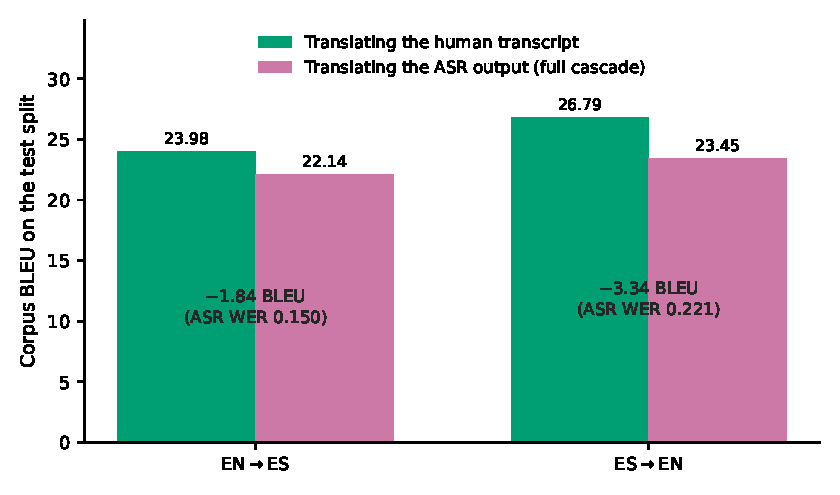
\includegraphics[width=\columnwidth]{figures/F_cascade_error.pdf}
\caption{Cost of automatic recognition in the cascade. Same translation model, same test
utterances, identical decoding; the only difference is whether the input is the human transcript
or the recogniser output.}
\label{fig:cascade}
\end{figure}

\subsection{Identity against the human ceiling}
Speaker similarity between source and synthesised output is $0.421$ (\ento) and $0.383$ (\esto).
The human cross-language anchor is $0.445$ in both directions, so the system retains
\textbf{94.5\,\%} and \textbf{86.1\,\%} of the achievable similarity (Fig.~\ref{fig:identity}).

\begin{figure}[!t]
\centering
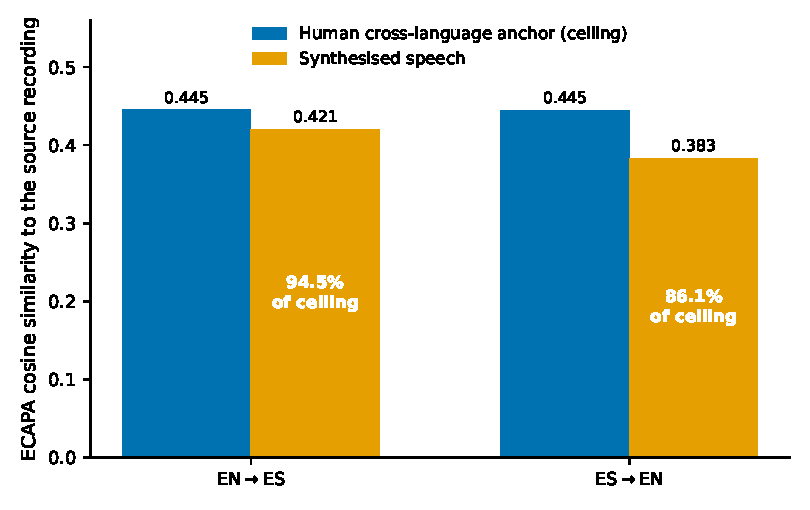
\includegraphics[width=\columnwidth]{figures/F_identity_ceiling.pdf}
\caption{Speaker identity against the human cross-language ceiling. The ceiling is the ECAPA cosine
between the source recording and the \emph{same speaker's} real recording in the other language.}
\label{fig:identity}
\end{figure}

Three points follow. The ceiling itself is low: two genuine recordings of one person in two
languages are only $0.445$ similar, so an evaluation that treats a raw cosine of $0.42$ as poor is
applying a standard human speech does not meet. The two ceilings are identical to three decimal
places, as they must be, since each compares the same pair of human recordings with the roles
exchanged; the asymmetry between 94.5\,\% and 86.1\,\% is therefore entirely in the synthesiser's
output, and cloning works better into Spanish than into English. Finally, per speaker the
percentage of ceiling ranges from 74.7\,\% to 147.2\,\% (\ento) and 55.5\,\% to 107.9\,\% (\esto);
values above 100\,\% arise where the synthesised audio inherits channel characteristics from the
reference clip that the human's second recording does not share.

\subsection{Cross-lingual prosody: human and system}
Table~\ref{tab:gap} reports the correspondence between each measure and the human target-language
recording, for the human re-enactment and for the system, pooled and within-speaker.
Fig.~\ref{fig:gap} plots the within-speaker columns.

\begin{table}[!t]
\caption{Cross-lingual prosody correspondence with the human target-language recording.
Within-speaker removes each speaker's own mean before correlating.}
\label{tab:gap}
\centering
\begin{tabular}{@{}lcccccc@{}}
\toprule
& \multicolumn{2}{c}{Human \enes{}} & \multicolumn{2}{c}{System \ento{}}
& \multicolumn{2}{c}{System \esto{}} \\
\cmidrule(lr){2-3}\cmidrule(lr){4-5}\cmidrule(lr){6-7}
Measure & Pool. & With. & Pool. & With. & Pool. & With. \\
\midrule
F0 level      & 0.952 & \textbf{0.849} & 0.698 & \textbf{0.311} & 0.754 & \textbf{0.314}\\
F0 range      & 0.263 & \textbf{0.214} & 0.142 & \textbf{0.035} & 0.132 & \textbf{0.040}\\
Duration      & 0.870 & \textbf{0.867} & 0.364 & \textbf{0.352} & 0.618 & \textbf{0.610}\\
Speaking rate & 0.595 & \textbf{0.601} & 0.360 & \textbf{0.372} & 0.353 & \textbf{0.346}\\
Energy        & ---   & ---            & 0.076 & \textbf{0.090} & 0.057 & \textbf{0.060}\\
\midrule
$n$ & \multicolumn{2}{c}{2{,}304} & \multicolumn{2}{c}{345--433} & \multicolumn{2}{c}{374--435}\\
\bottomrule
\end{tabular}
\end{table}

\begin{figure}[!t]
\centering
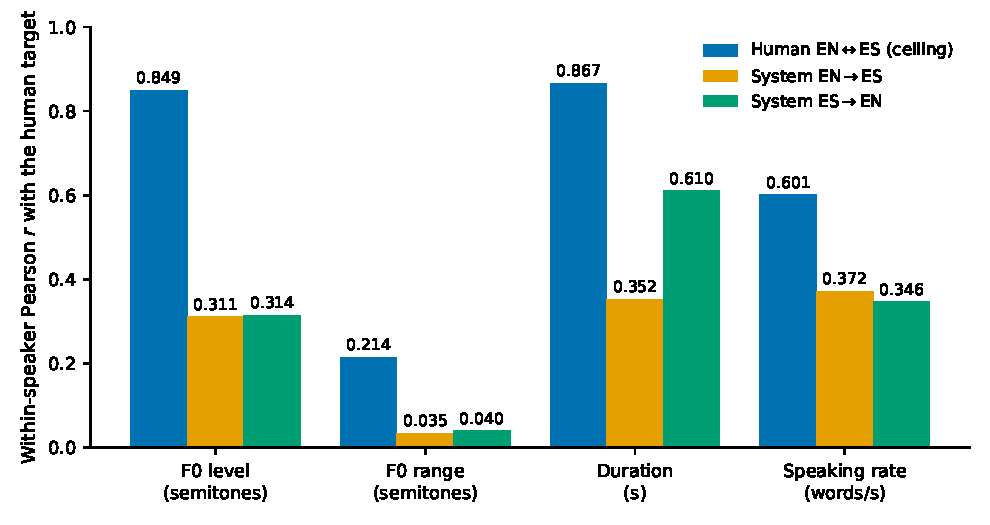
\includegraphics[width=\columnwidth]{figures/F_prosody_gap.pdf}
\caption{Within-speaker cross-lingual prosody correspondence. Blue: what a human achieves
re-enacting their own utterance in the other language. Orange and green: what the system achieves
against that same human recording.}
\label{fig:gap}
\end{figure}

A human reproduces their own pitch level across languages at $r=0.849$ within-speaker; the system
reaches $0.311$ and $0.314$, about 37\,\% of the human figure. Pitch range collapses from an
already modest human $0.214$ to $0.035$ and $0.040$: the utterance-level variation that
distinguishes an animated turn from a flat one does not survive. Duration survives best
($0.352$ and $0.610$ against $0.867$), which is expected since utterance length is largely
determined by content. Energy carries essentially nothing, as expected for a quantity dominated by
recording gain.

\subsection{Why pooled correlations must not be quoted alone}
For the system's pitch level the pooled correlation is $0.698$ and $0.754$, while within-speaker it
is $0.311$ and $0.314$; the between-speaker correlation is $0.895$ and $0.847$, and speaker
differences account for 47\,\% and 61\,\% of total variance (Fig.~\ref{fig:pooled}).

\begin{figure}[!t]
\centering
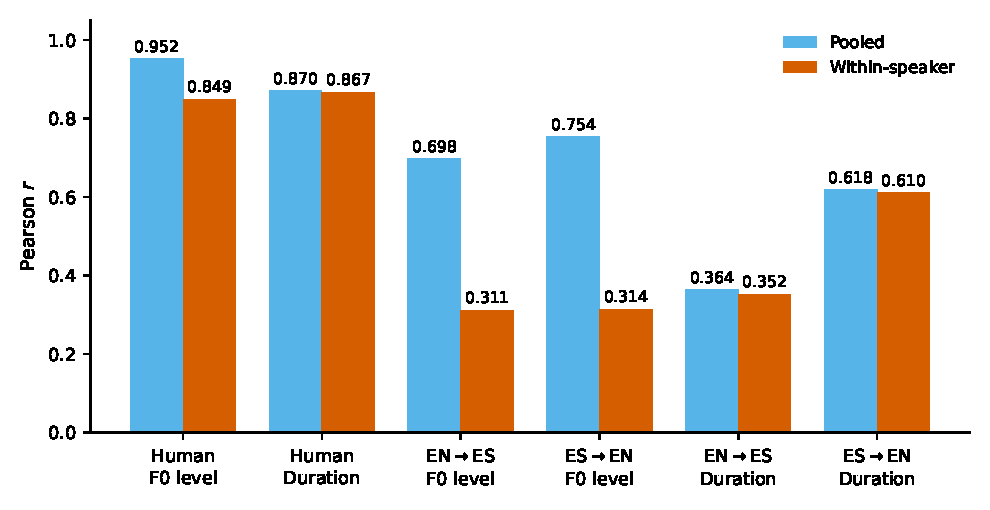
\includegraphics[width=\columnwidth]{figures/F_pooled_vs_within.pdf}
\caption{Pooled against within-speaker correlation. Where the two diverge, most of the pooled
figure is stable between-speaker variation carried by voice cloning rather than prosody transfer.}
\label{fig:pooled}
\end{figure}

A pooled correlation near $0.75$ would ordinarily be reported as strong prosody transfer. It is not:
it is the voice clone reproducing the speaker's habitual pitch, which is the identity result of
Section~IV-B appearing again under a different name. Reporting the pooled figure alone attributes
the success of one component to another.

\subsection{Is target-language prosody predictable?}
Table~\ref{tab:ridge} gives the test-split result. Pitch level is not predictable beyond the
baseline: the improvement is $-0.02\,\%$ and $-0.00\,\%$, and the regulariser selected
$\lambda=10^{6}$, at which every weight vanishes, so the model reduced itself to B2. Pitch range is
predictable in both directions, by $5.14\,\%$ and $3.89\,\%$ mean absolute error, with
speaker-clustered $p$ of $0.0012$ and $0.0001$ and bootstrap intervals excluding zero. The duration
ratio is not reliably predictable.

\begin{table}[!t]
\caption{Prosody prediction on the held-out test split (mean absolute error; lower is better).
$p$ is a Wilcoxon test on per-speaker mean absolute errors, $n=14$ speakers.}
\label{tab:ridge}
\centering
\begin{tabular}{@{}llrrrrr@{}}
\toprule
Dir. & Target & B1 & B0 & B2 & Ridge & $\Delta$B2 ($p$)\\
\midrule
\ento & F0 level  & 5.783 & 1.375 & 1.353 & 1.353 & $-0.02\,\%$ (.0040)\\
\ento & F0 range  & 1.034 & 0.977 & 0.983 & \textbf{0.932} & $-5.14\,\%$ (.0012)\\
\ento & Dur.\ ratio & 0.181 & 0.186 & 0.181 & 0.180 & $-0.73\,\%$ (.194)\\
\esto & F0 level  & 5.947 & 1.350 & 1.329 & 1.329 & $-0.00\,\%$ (.903)\\
\esto & F0 range  & 1.017 & 0.963 & 0.968 & \textbf{0.931} & $-3.89\,\%$ (.0001)\\
\esto & Dur.\ ratio & 0.182 & 0.187 & 0.182 & 0.172 & $-5.34\,\%$ (.104)\\
\bottomrule
\end{tabular}
\end{table}

Under Bonferroni at $\alpha=0.05$ the threshold is $0.0083$, and three of six $p$-values fall below
it; the same three survive Holm and Benjamini--Hochberg. Only two are practically meaningful, the
pitch-range results. The third, \ento{} pitch level, has an effect of $-0.02\,\%$: a signed-rank
test over near-identical error vectors can return a small $p$ for a zero-sized effect, and we
report it so that it cannot be quoted as a third success.

The mechanism is in the coefficients. The weight on source F0 range is $-0.191$ (\ento) and
$-0.143$ (\esto), large relative to the other five and \emph{negative}: an unusually wide source
pitch range should be predicted narrower in the target. Per-utterance variation regresses towards
the speaker's habitual range rather than transferring one for one. A conditioning mechanism that
copied source pitch directly into the target would copy the wrong thing.

\subsection{Duration inflation}
Synthesised utterances run $1.52\times$ longer than the human target on average (4.07\,s against
2.67\,s); the median per-utterance ratio is $1.43$ and 25.1\,\% exceed $2.0\times$
(Fig.~\ref{fig:dur}). The inflation is systematic, not random, and it is fatal for dubbing: at
$1.5\times$ per utterance a dubbed track loses synchronisation within a few turns.

\begin{figure}[!t]
\centering
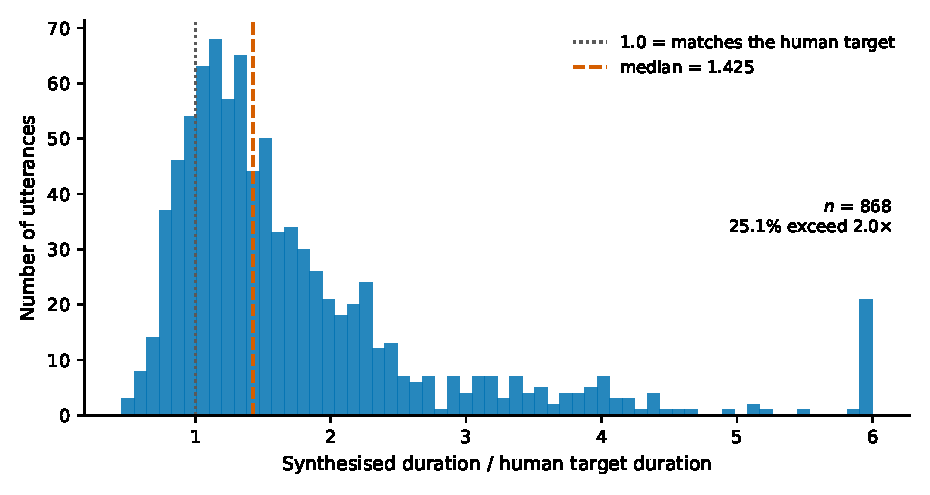
\includegraphics[width=\columnwidth]{figures/F_duration_ratio.pdf}
\caption{Ratio of synthesised to human-target duration over 868 utterances, clipped at $6\times$
for display.}
\label{fig:dur}
\end{figure}

We built a video dubbing application that time-scales each synthesised segment to the slot it
replaces using WORLD analysis and resynthesis \cite{morise2016world}, with scaling clamped to
$0.5$--$2.0\times$. Over five jobs and 83 segments, the dubbed track lands within 7\,\% of the
original length where the raw length ratio is at or below about $1.6\times$; at $2.17\times$ the
clamp binds on 59\,\% of segments and the output degrades. No amount of signal processing absorbs a
$2.17\times$ ratio: the constraint is upstream, in a translation whose spoken length was never
controlled, which is exactly the problem length-aware translation for dubbing addresses
\cite{lakew2021verbosity,federico2020dubbing}.

% =======================================================================================
\section{Discussion}

\subsection{A measurement pitfall, quantified}
\label{sec:pitfall}
An earlier version of this analysis reported that the system transferred essentially no pitch
information, $r=0.090$. Two defects produced that figure. Correlating pitch in hertz lets values
furthest from the mean dominate, and a single octave-doubled observation destroys the statistic;
correlating in semitones on identical measurements moved \ento{} F0 from $0.048$ to $0.368$.
Adding the plausibility gate of Section~\ref{sec:bands} moved the same figure from $0.368$ to
$0.820$.

A third intervention, attempted first, made matters worse. Narrowing the estimator's \emph{search}
band to 60--400\,Hz appears to be the natural remedy for octave errors; measured, it was the worst
of four bands (generated-versus-human F0 correlation, semitone space, gated: $0.371/0.589$ for
60--400\,Hz; $0.778/0.739$ for 65--600; $0.888/0.856$ for 65--1000; $0.822/0.819$ for 65--2093).
The cause is that a narrow band starves the voiced/unvoiced decision of candidates: one test file
went from ten voiced frames to zero. The correct design separates a wide search band from a narrow
downstream plausibility gate. We report this because the erroneous number was the more publishable
one, and because the plausible fix was the wrong fix.

\subsection{Interpretation}
The two headline results diverge because of the architecture, not because of an implementation
defect. The speaker embedding on which zero-shot cloning depends is trained for verification and is
designed to be invariant to what a speaker does on any particular utterance. A system built on such
an embedding will reproduce \emph{who} is speaking and discard \emph{how} they spoke. Closing that
gap requires an additional conditioning path, which is what expressive dubbing systems build
\cite{swiatkowski2023dubbing,song2023styles2st}.

The prediction experiment qualifies this constructively. Cross-lingual prosody is not arbitrary,
but its predictable component is narrower than one might hope, and compressive rather than
one-for-one.

\subsection{Limitations}
No listening study was conducted; all results are instrumental, and whether listeners perceive the
prosody gap as strongly as the correlations imply is untested. The study covers one corpus, one
language pair and 14 test speakers, which is why speaker-clustered inference is used throughout.
The corpus's target side is a re-enactment rather than a literal translation, so translation scores
against it are conservative. Prosody is characterised by utterance-level statistics, which do not
capture contour shape; a frame-level comparison under dynamic time warping would be a stronger
instrument and would make these figures directly comparable with published expressive-dubbing
scores. Finally, the prosody model is analysis, not control: it predicts target-language prosody but
does not condition the synthesiser.

% =======================================================================================
\section{Conclusion}
A same-speaker parallel corpus converts cross-lingual synthesis evaluation from a set of
uncalibrated similarity scores into a comparison against what the same person actually did. Under
that comparison the answer is specific: current zero-shot cross-lingual voice cloning carries the
speaker but not the speech act. Identity survives at 86--95\,\% of the human cross-language ceiling;
within-speaker pitch level survives at roughly a third of the human figure and pitch range at
essentially none. The predictable part of cross-lingual prosody lies in pitch range, and the
relationship is compressive. Future work should validate these instrumental findings with a
listening study, replace utterance-level statistics with warped frame-level contour comparison, and
close the loop by using the prosody prediction to condition synthesis.

% =======================================================================================
\section*{Acknowledgment}
The authors thank E.~M.~U.~W.~J.~B.~Ekanayake and H.~P.~D.~P.~Pathirana for supervision, and
N.~G.~Ward and colleagues at the University of Texas at El Paso for releasing the DRAL corpus into
the public domain.

\bibliographystyle{IEEEtran}
\bibliography{references}

\end{document}
